\documentclass{ximera}
\author{Jim Talamo}
\newcommand{\RR}{\mathbb R}
\renewcommand{\d}{\,d}
\newcommand{\dd}[2][]{\frac{d #1}{d #2}}
\renewcommand{\l}{\ell}
\newcommand{\ddx}{\frac{d}{dx}}
\newcommand{\dfn}{\textbf}
\newcommand{\eval}[1]{\bigg[ #1 \bigg]}


\title[Dig-In:]{Remainders}

\outcome{Define the remainder for a convergent series.}
\outcome{Estimate the value of a convergent series using the sequence of partial sums.}
\outcome{Explain the relationship between the remainder of a convergent series and the sequence of partial sums.}

\begin{document}
\begin{abstract}
  We can approximate the value of convergent series using the sequence of partial sums.
\end{abstract}
\maketitle

Given a series $\sum_{k=n_0}^{\infty} a_k$, our attempt to determine whether it converges or diverges requires that we consider the limit of the corresponding sequence of partial sums $\{s_n\}_{n = n_0}$, whose terms are given by $s_n = \sum_{k=n_0}^{n}  a_k$.   For geometric and telescoping series, we were able to find an explicit formula for the terms in the sequence of partial sums then analyze the limit directly.  We have now seen that this is not always possible, but thankfully, we have developed a few tests that allow us to determine whether this limit exists.  However, this leads to an important question.

\begin{quote}
Once we have established that a series converges, how can we determine its value?
\end{quote}

If we aren't able to find an explicit formula for $s_n$, we likely will not be able to find the exact value of the series.  For most practical applications that arise in science and engineering,  we really do not need to find the exact value of a convergent series; we only need to know the value to within a predetermined margin of error.

%%%%%%%%%%%%%%%%%%%%%%%%%%%%%%%%%%%%%%%%%%%%%%%%%%%%%%%%%%%%%%%%%%%%%

\section{Remainders}

For a series $\sum_{k=1}^{\infty} a_k$, we may write the following.

\begin{align*}
\sum_{k=1}^\infty a_k &= a_1+a_2+\ldots+a_n + a_{n+1} + a_{n+2}+ \ldots\\
\sum_{k=1}^\infty a_k &= \bigg[a_1+a_2+\ldots+a_n\big] + \big[a_{n+1} + a_{n+2}+ \ldots \bigg]\\
\sum_{k=1}^\infty a_k &= \sum_{k=1}^n a_k+\sum_{k=n+1}^\infty a_k \\
\sum_{k=1}^\infty a_k &= s_n+\sum_{k=n+1}^\infty a_k
\end{align*}

Note that $\sum_{k=1}^n a_k$ is precisely $s_n$.  Note that for every value of $n$, $s_n$ must be finite since the sum that defines it is the sum of finitely many terms.  Keeping this in mind, notice the following.

\begin{itemize}
\item If $\sum_{k=1}^\infty a_k$ diverges, then $\sum_{k=n+1}^\infty a_k$ \wordChoice{\choice[correct]{must diverge}\choice{could converge or diverge}\choice{must converge}} since the lower index of summation \wordChoice{\choice{affects}\choice[correct]{does not affect}} whether a series converges or diverges .
\item If $\sum_{k=1}^\infty a_k$ converges, then $\sum_{k=n+1}^\infty a_k$ \wordChoice{\choice{must diverge}\choice{could converge or diverge}\choice[correct]{must converge}} since the lower index of summation \wordChoice{\choice{affects}\choice[correct]{does not affect}} whether a series converges or diverges .
\end{itemize}

Now, if the series converges, $\sum_{k=1}^\infty a_k  = \lim_{n \to \infty} s_n$ by definition, which means that the terms in the sequence $\{s_n\}_{n=1}$ should become as close as we want to the value of the series for all large enough values of $n$.  This means that we can approximate the value of $\sum_{k=1}^\infty a_k$ by using terms in the sequence of partial sums!  

\begin{remark}
Note that for a specified value of $n$, we could also compute $s_n$ for a divergent series, but this is inherently meaningless since there is no value associated to $\sum_{k=1}^\infty a_k$ if it diverges.
\end{remark}

Now that we have an estimate, the next important question to ask is: just how good is this estimate?  This is where the idea of a \emph{remainder} comes in.

\begin{definition}
Given a convergent series $\sum_{k=n_0}^{\infty} a_k$, we define the sequence of remainders $\{r_n\}_{n=1}$ by 
\[
r_n := \sum_{k=n+1}^{\infty} a_k
\]
for all $n \geq 1$.
\end{definition}

Note that $r_n$ is also an infinite series, and its index starts at $n+1$.  The reason for this choice is that it allows us to split up a \emph{convergent} series in a useful way.  

\begin{image}
  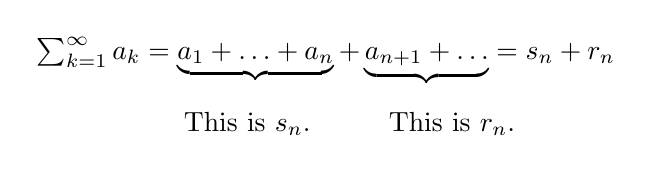
\begin{tikzpicture}
        \node at (0,0) {
          $ \sum_{k=1}^{\infty} a_k=\underbrace{a_1+\ldots +a_n}+ \underbrace{a_{n+1}+ \ldots} = s_n+r_n$};
        \node at (1.6,-.8) { This is $r_n$.};
       
        \node at (-1,-.8) { This is $s_n$. };
        
      \end{tikzpicture}
  \end{image}



\begin{remark}
Note that in general, we can repeat this construction in this section for any convergent series for which the lower index is $n_0$.

\begin{align*}
\sum_{k=n_0}^\infty a_k &= \sum_{k=n_0}^n a_k+\sum_{k=n+1}^\infty a_k,
\end{align*}

where $n \geq n_0$.  The sequence of remainders $\{r_n\}_{n=n_0}$ is then defined by the formula $r_n = \sum_{k=n+1}^{\infty} a_k$ for $n \geq n_0$ (rather than for $n \geq 1$) . 
\end{remark}

\begin{example}
Consider the series $\sum_{k=1}^{\infty} \frac{1}{k^2}$.  It can be shown that this series converges, but $\sum_{k=1}^{\infty} \frac{1}{k^2}$ \wordChoice{\choice{is}\choice[correct]{is not}} a geometric series and is not a telescoping series.  As such, we will be hard pressed to find its exact value.

I. By using the first four terms of this series, approximate its value.

\begin{explanation}
We will approximate the value of this series by 

\begin{align*}
s_4 &= \frac{1}{1^2}+\frac{1}{2^2}+\frac{1}{3^2}+\frac{1}{4^2} =1+\frac{1}{4}+\frac{1}{9}+\frac{1}{16} \\
&  = \answer[tolerance=.001]{1.4236} \textrm{ (to four decimal places) }
\end{align*}


II. Given that $\sum_{k=1}^{\infty} \frac{1}{k^2} = \frac{\pi^2}{6}$, we can use the above result to find \wordChoice{\choice{$r_3$}\choice[correct]{$r_4$}\choice{$r_5$}}.  By noting that 

\[
\sum_{k=1}^{\infty} \frac{1}{k^2} = s_4+r_4,
\]
we find that $r_4 = \frac{\pi^2}{6} - s_4 = .2213$ to four decimal places.
\end{explanation}

\end{example}

\begin{remark}
Finding the exact value of the series $\sum_{k=1}^{\infty}$ is not easy!  In fact, this problem was first posed by the Italian mathematician Pietro Mengoli in 1650 and became known as the Basel problem. The problem remained unsolved until 1734 by the famous mathematician Leonard Euler.  
\end{remark}

%%%%%%%%%%%%%%%%%%%%%%%%%%%%%%%%%%%%%%%%%%%%%%%%%%%%%%%%%%%%%%%%%%%%%%

\section{The remainder as ``error''}

When we want to approximate the value of a convergent series $\sum_{k=1}^{\infty} a_k$ by the finite sum $\sum_{k=1}^{n} a_k$, we generally want $\sum_{k=1}^{n} a_k$ to be very ``close'' to the value of the infinite series where, ``close'' will vary from application to application.  However, this idea gives a good conceptual interpretation of the remainder.

\begin{image}
  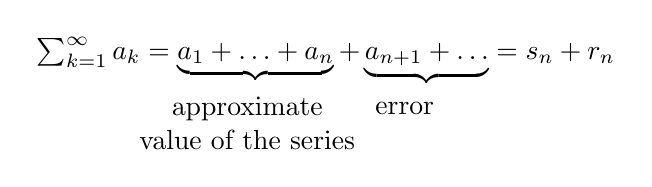
\begin{tikzpicture}
        \node at (0,0) {
          $ \sum_{k=1}^{\infty} a_k=\underbrace{a_1+\ldots +a_n}+ \underbrace{a_{n+1}+ \ldots} = s_n+r_n$};
        \node at (1,-.6) { error};
       
        \node at (-1,-.6) {approximate };
        \node at (-1,-1) {value of the series };
                
      \end{tikzpicture}
  \end{image}

We thus can think about $r_n$ as the error made when approximating the value of the\emph{infinite} series $\sum_{k=1}^{\infty} a_k$ by the \emph{finite} sum $\sum_{k=1}^{n} a_k$.

\begin{example}
Suppose that $\{a_n\}_{n=1}$ is a sequence and it is known that $\sum_{k=1}^{n} a_k = \frac{2n}{n+1}$.  Explain why we can define a sequence of remainders for the infinite series $\sum_{k=1}^{\infty} a_k$, then find an explicit formula for $s_n$ and $r_n$.

\begin{explanation}
Note that we are actually given that $s_n = \frac{2n}{n+1}$.  Since $\lim_{n \to \infty} s_n = \answer{2}$, we have that $\sum_{k=1}^{\infty} a_k$ \wordChoice{\choice{diverges}\choice{converges to $2$}} .

Since the series \wordChoice{\choice{diverges}\choice{converges}}, we may define a sequence of remainders $\{r_n\}_{n=1}$.  Furthermore, notice that the relationship $\sum_{k=1}^{\infty} a_k = s_n+r_n$ allows us to find an explicit formula for $r_n$.

\begin{align*}
\sum_{k=1}^{\infty} a_k &= s_n+r_n \\
2 &= \frac{2n}{n+1}+r_n \\
r_n &= 2-\frac{2n}{n+1}
\end{align*}

\end{explanation}

What is the smallest integer $N$ so $\sum_{k=1}^{N} a_k$ is within $.01$ of the exact value of $\sum_{k=1}^{\infty} a_k$?

\begin{explanation}
Notice that this question is really asking how many terms we need in a finite sum to ensure that the computed value will be accurate to $.01$ of the exact value of the infinite series.  Since $r_N$ will measure the error resulting from approximating the infinite series by $s_N$, we find $N$ by setting $r_N \leq .01$.

\begin{align*}
2-\frac{2N}{N+1} &\leq \frac{1}{100} \\
200-\frac{200N}{N+1} & \leq 1 \\
\frac{200N}{N+1} & \geq 199 \\
200N & \geq 199N+199 \\
N \geq 199
\end{align*}

We thus know that $s_{199}$ can be used to approximate the value of $\sum_{k=1}^{\infty} a_k$ to within $.01$ of its exact value.
\end{explanation}

\end{example}

\section{Remainders and convergence}

In the last example, $r_n = 2-\frac{2n}{n+1}$, and we can compute readily that $\lim_{n \to \infty} r_n = \answer{0}$.  This leads to an interesting question.

\begin{question}
If $\sum_{k=n_0}^\infty a_k$ converges, must $\lim_{n \to \infty} r_n =0$?
\end{question}

The answer is yes!  If $\sum_{k=n_0}^\infty a_k$ converges, call its value $S$.  Since $\sum_{k=n_0}^\infty a_k$ converges, by definition, we have that $\lim_{n \to \infty} s_n = \answer{S}$.  

By considering the relationship $ \sum_{k=1}^{\infty} a_k = s_n+r_n$ and substituting $ \sum_{k=1}^{\infty} a_k =S$, we may write 

\[ r_n = S - s_n. \\
\]

Taking limits of both sides gives us the desired result.

\begin{align*}
\lim_{n \to \infty} r_n &= \lim_{n \to \infty} \bigg(S- s_n\bigg) \\
\lim_{n \to \infty} r_n &= \lim_{n \to \infty} S- \lim_{n \to \infty} s_n \\
\lim_{n \to \infty} r_n &= S- S  \\
 \lim_{n \to \infty} r_n  &= 0
\end{align*}

Thus, if $\sum_{k=n_0}^{\infty} a_k$ converges, then we must have that $\lim_{n \to 0} r_n =0$.  Conceptually, this should not be surprising since this means that as we use larger and larger values for $n$, the terms $s_n$ approximate the value of the series more closely since the error will approach $0$. 

As it turns out, the converse of the statement in the last paragraph is also true, but showing it requires a more technical argument that relies on the formal definition of the limit of a sequence.  Instead of providing the details, we state the following important theorem.  

\begin{theorem}[Remainders and Convergence]\index{remainders and convergence}
Consider the series $\sum_{k=n_0}^{\infty} a_k$ and for every $n \geq n_0$, define $r_n = \sum_{k=n+1}^{\infty} a_k$.  Then, $\sum_{k=n_0}^{\infty} a_k$ converges if and only if $\lim_{n \to \infty} r_n =0$.
\end{theorem}


\end{document}
